
\chapter{Fractions Décimales}
{https://sacado.xyz/qcm/parcours_show_course/0/117125}
{


 \begin{CpsCol}
 \section{Les savoir-faire du parcours}
 \begin{itemize}
 \item Savoir écrire une fraction décimale.
 \item Savoir compléter une égalité de fractions décimales.
 \item Savoir comparer une fraction décimale à l'unité.
 \item Savoir décomposer une fraction décimale.
 \item Savoir encadrer une fraction décimale par deux entiers consécutifs.
 \item Savoir ajouter des fractions décimales.
 \item Savoir utiliser des fractions décimales.
 \item Savoir repérer une fraction décimale sur une demi-droite graduée.
 \item Savoir placer une fraction décimale sur une demi-droite graduée.
 \end{itemize}
 \end{CpsCol}
}

\begin{pageCours} 

\section{Partage de l'unité en base 10}

\begin{DefT}{Dixième. centième. Millièmes}
\begin{itemize}[leftmargin=*]
\item Lorsqu'on partage l'\textbf{unité} en \textbf{dix parties égales}, on obtient dix \textbf{dixièmes}.
\item Lorsqu'on partage chaque \textbf{dixième de l'unité} en \textbf{dix parties égales}, l'unité est partagée en \textbf{cent parties égales} et on obtient \textbf{cent centièmes}.
\item En poursuivant ainsi des partages en dix, on obtient des \textbf{millièmes}, des \textbf{dix-millièmes}...
\end{itemize}
\begin{center}
\begin{tikzpicture}[line cap=round,line join=round,>=triangle 45,x=1.5cm,y=1.5cm]
%\clip(-0.10372640678354844,-1.2256531369507317) rectangle (10.114725141662657,2.104805145505822);
\fill[line width=2.pt,color=qqqqff,fill=qqqqff,fill opacity=0.10000000149011612] (0.,0.) -- (10.,0.) -- (10.,1.) -- (0.,1.) -- cycle;
\fill[line width=2.pt,color=qqwuqq,fill=qqwuqq,fill opacity=0.10000000149011612] (0.,0.) -- (0.,-1.) -- (10.,-1.) -- (10.,0.) -- cycle;
\fill[line width=2.pt,color=zzttqq,fill=zzttqq,fill opacity=0.10000000149011612] (0.,1.) -- (0.,2.) -- (10.,2.) -- (10.,1.) -- cycle;
\draw [line width=2.pt,color=qqqqff] (0.,0.)-- (10.,0.);
\draw [line width=2.pt,color=qqqqff] (10.,0.)-- (10.,1.);
\draw [line width=2.pt,color=qqqqff] (10.,1.)-- (0.,1.);
\draw [line width=2.pt,color=qqqqff] (0.,1.)-- (0.,0.);
\draw [line width=2.pt,color=qqwuqq] (0.,0.)-- (0.,-1.);
\draw [line width=2.pt,color=qqwuqq] (0.,-1.)-- (10.,-1.);
\draw [line width=2.pt,color=qqwuqq] (10.,-1.)-- (10.,0.);
\draw [line width=2.pt,color=qqwuqq] (10.,0.)-- (0.,0.);
\draw [line width=2.pt,color=zzttqq] (1.,1.)-- (1.,-1.);
\draw [line width=2.pt,color=zzttqq] (2.,1.)-- (2.,-1.);
\draw [line width=2.pt,color=zzttqq] (3.,1.)-- (3.,-1.);
\draw [line width=2.pt,color=zzttqq] (4.,1.)-- (4.,-1.);
\draw [line width=2.pt,color=zzttqq] (5.,1.)-- (5.,-1.);
\draw [line width=2.pt,color=zzttqq] (6.,1.)-- (6.,-1.);
\draw [line width=2.pt,color=zzttqq] (7.,1.)-- (7.,-1.);
\draw [line width=2.pt,color=zzttqq] (8.,1.)-- (8.,-1.);
\draw [line width=2.pt,color=zzttqq] (9.,1.)-- (9.,-1.);
\draw [line width=2.pt,color=zzttqq] (0.5,0.)-- (0.5,-1.);
\draw [line width=2.pt,color=zzttqq] (1.5,0.)-- (1.5,-1.);
\draw [line width=2.pt,color=zzttqq] (2.5,0.)-- (2.5,-1.);
\draw [line width=2.pt,color=zzttqq] (3.5,0.)-- (3.5,-1.);
\draw [line width=2.pt,color=zzttqq] (4.5,0.)-- (4.5,-1.);
\draw [line width=2.pt,color=zzttqq] (5.5,0.)-- (5.5,-1.);
\draw [line width=2.pt,color=zzttqq] (6.5,0.)-- (6.5,-1.);
\draw [line width=2.pt,color=zzttqq] (7.5,0.)-- (7.5,-1.);
\draw [line width=2.pt,color=zzttqq] (8.5,0.)-- (8.5,-1.);
\draw [line width=2.pt,color=zzttqq] (9.5,0.)-- (9.5,-1.);
\draw [line width=2.pt,color=zzttqq] (0.1,0.)-- (0.1,-1.);
\draw [line width=2.pt,color=zzttqq] (0.2,0.)-- (0.2,-1.);
\draw [line width=2.pt,color=zzttqq] (0.3,0.)-- (0.3,-1.);
\draw [line width=2.pt,color=zzttqq] (0.4,0.)-- (0.4,-1.);
\draw [line width=2.pt,color=zzttqq] (0.6,0.)-- (0.6,-1.);
\draw [line width=2.pt,color=zzttqq] (0.7,0.)-- (0.7,-1.);
\draw [line width=2.pt,color=zzttqq] (0.8,0.)-- (0.8,-1.);
\draw [line width=2.pt,color=zzttqq] (0.9,0.)-- (0.9,-1.);
\draw [line width=2.pt,color=zzttqq] (1.1,0.)-- (1.1,-1.);
\draw [line width=2.pt,color=zzttqq] (1.2,0.)-- (1.2,-1.);
\draw [line width=2.pt,color=zzttqq] (1.3,0.)-- (1.3,-1.);
\draw [line width=2.pt,color=zzttqq] (1.4,0.)-- (1.4,-1.);
\draw [line width=2.pt,color=zzttqq] (1.6,0.)-- (1.6,-1.);
\draw [line width=2.pt,color=zzttqq] (1.7,0.)-- (1.7,-1.);
\draw [line width=2.pt,color=zzttqq] (1.8,0.)-- (1.8,-1.);
\draw [line width=2.pt,color=zzttqq] (1.9,0.)-- (1.9,-1.);
\draw [line width=2.pt,color=zzttqq] (2.1,0.)-- (2.1,-1.);
\draw [line width=2.pt,color=zzttqq] (2.2,0.)-- (2.2,-1.);
\draw [line width=2.pt,color=zzttqq] (2.3,0.)-- (2.3,-1.);
\draw [line width=2.pt,color=zzttqq] (2.4,0.)-- (2.4,-1.);
\draw [line width=2.pt,color=zzttqq] (2.6,0.)-- (2.6,-1.);
\draw [line width=2.pt,color=zzttqq] (2.7,0.)-- (2.7,-1.);
\draw [line width=2.pt,color=zzttqq] (2.8,0.)-- (2.8,-1.);
\draw [line width=2.pt,color=zzttqq] (2.9,0.)-- (2.9,-1.);
\draw [line width=2.pt,color=zzttqq] (3.1,0.)-- (3.1,-1.);
\draw [line width=2.pt,color=zzttqq] (3.2,0.)-- (3.2,-1.);
\draw [line width=2.pt,color=zzttqq] (3.3,0.)-- (3.3,-1.);
\draw [line width=2.pt,color=zzttqq] (3.4,0.)-- (3.400212563855043,-0.9870631983522774);
\draw [line width=2.pt,color=zzttqq] (3.6,0.)-- (3.6,-1.);
\draw [line width=2.pt,color=zzttqq] (3.7,0.)-- (3.7,-1.);
\draw [line width=2.pt,color=zzttqq] (3.8,0.)-- (3.8,-1.);
\draw [line width=2.pt,color=zzttqq] (3.9,0.)-- (3.9,-1.);
\draw [line width=2.pt,color=zzttqq] (4.1,0.)-- (4.1,-1.);
\draw [line width=2.pt,color=zzttqq] (4.2,0.)-- (4.2,-1.);
\draw [line width=2.pt,color=zzttqq] (4.3,0.)-- (4.3,-1.);
\draw [line width=2.pt,color=zzttqq] (4.4,0.)-- (4.4,-1.);
\draw [line width=2.pt,color=zzttqq] (4.6,0.)-- (4.6,-1.);
\draw [line width=2.pt,color=zzttqq] (4.7,0.)-- (4.7,-1.);
\draw [line width=2.pt,color=zzttqq] (4.8,0.)-- (4.8,-1.);
\draw [line width=2.pt,color=zzttqq] (4.9,0.)-- (4.9,-1.);
\draw [line width=2.pt,color=zzttqq] (5.1,0.)-- (5.1,-1.);
\draw [line width=2.pt,color=zzttqq] (5.2,0.)-- (5.2,-1.);
\draw [line width=2.pt,color=zzttqq] (5.3,0.)-- (5.3,-1.);
\draw [line width=2.pt,color=zzttqq] (5.4,0.)-- (5.4,-1.);
\draw [line width=2.pt,color=zzttqq] (5.6,0.)-- (5.6,-1.);
\draw [line width=2.pt,color=zzttqq] (5.7,0.)-- (5.7,-1.);
\draw [line width=2.pt,color=zzttqq] (5.8,0.)-- (5.8,-1.);
\draw [line width=2.pt,color=zzttqq] (5.9,0.)-- (5.9,-1.);
\draw [line width=2.pt,color=zzttqq] (6.1,0.)-- (6.1,-1.);
\draw [line width=2.pt,color=zzttqq] (6.2,0.)-- (6.2,-1.);
\draw [line width=2.pt,color=zzttqq] (6.3,0.)-- (6.3,-1.);
\draw [line width=2.pt,color=zzttqq] (6.4,0.)-- (6.4,-1.);
\draw [line width=2.pt,color=zzttqq] (6.6,0.)-- (6.6,-1.);
\draw [line width=2.pt,color=zzttqq] (6.7,0.)-- (6.7,-1.);
\draw [line width=2.pt,color=zzttqq] (6.8,0.)-- (6.8,-1.);
\draw [line width=2.pt,color=zzttqq] (6.9,0.)-- (6.9,-1.);
\draw [line width=2.pt,color=zzttqq] (7.1,0.)-- (7.1,-1.);
\draw [line width=2.pt,color=zzttqq] (7.2,0.)-- (7.2,-1.);
\draw [line width=2.pt,color=zzttqq] (7.3,0.)-- (7.3,-1.);
\draw [line width=2.pt,color=zzttqq] (7.4,0.)-- (7.4,-1.);
\draw [line width=2.pt,color=zzttqq] (7.6,0.)-- (7.6,-1.);
\draw [line width=2.pt,color=zzttqq] (7.7,0.)-- (7.7,-1.);
\draw [line width=2.pt,color=zzttqq] (7.8,0.)-- (7.8,-1.);
\draw [line width=2.pt,color=zzttqq] (7.9,0.)-- (7.9,-1.);
\draw [line width=2.pt,color=zzttqq] (8.1,0.)-- (8.1,-1.);
\draw [line width=2.pt,color=zzttqq] (8.2,0.)-- (8.2,-1.);
\draw [line width=2.pt,color=zzttqq] (8.3,0.)-- (8.3,-1.);
\draw [line width=2.pt,color=zzttqq] (8.4,0.)-- (8.4,-1.);
\draw [line width=2.pt,color=zzttqq] (8.6,0.)-- (8.6,-1.);
\draw [line width=2.pt,color=zzttqq] (8.7,0.)-- (8.7,-1.);
\draw [line width=2.pt,color=zzttqq] (8.8,0.)-- (8.8,-1.);
\draw [line width=2.pt,color=zzttqq] (8.9,0.)-- (8.9,-1.);
\draw [line width=2.pt,color=zzttqq] (9.1,0.)-- (9.1,-1.);
\draw [line width=2.pt,color=zzttqq] (9.2,0.)-- (9.2,-1.);
\draw [line width=2.pt,color=zzttqq] (9.3,0.)-- (9.3,-1.);
\draw [line width=2.pt,color=zzttqq] (9.4,0.)-- (9.4,-1.);
\draw [line width=2.pt,color=zzttqq] (9.6,0.)-- (9.6,-1.);
\draw [line width=2.pt,color=zzttqq] (9.7,0.)-- (9.7,-1.);
\draw [line width=2.pt,color=zzttqq] (9.8,0.)-- (9.8,-1.);
\draw [line width=2.pt,color=zzttqq] (9.9,0.)-- (9.9,-1.);
\draw [line width=2.pt,color=zzttqq] (0.,1.)-- (0.,2.);
\draw [line width=2.pt,color=zzttqq] (0.,2.)-- (10.,2.);
\draw [line width=2.pt,color=zzttqq] (10.,2.)-- (10.,1.);
\draw [line width=2.pt,color=zzttqq] (10.,1.)-- (0.,1.);
\draw [color=zzttqq](4.6,1.5522518395528027) node[anchor=north west] {Unité};
\draw [color=qqqqff](0.05202709156976383,0.5455451314466172) node[anchor=north west] {Dixième};
\draw [color=qqwuqq](0.024950390493181537,-1.0) node[anchor=north west] {Centième};
\end{tikzpicture}
\end{center}
\end{DefT}


\section{Fractions décimales}

\begin{Def}
Une fraction décimale est une fraction dont le dénominateur est égal à $1$ ; $10$ ; $100$ ; $1000$...

ou tout autre nombre qui s'écrit sous la forme $10\times10\times...\times10$
\end{Def}

\begin{Ex}
Le nombre \textbf{soixante-trois-dixièmes} s'écrit $\frac{63}{10}$.
\end{Ex}



\section{Décomposer une fraction décimale}


\begin{Def}
Une \textbf{fraction décimale} peut se décomposer sous la forme de la somme d'un \textbf{nombre entier} et d'une \textbf{fraction décimale} plus \textbf{petite que 1}.
\end{Def}

\begin{Ex}
La fraction décimale $\frac{866}{10}$ peut se décomposer sous la forme suivante :
\[\frac{866}{10}=86+\frac{6}{10}\]
\end{Ex}

\end{pageCours} 


\begin{pageAD} 
 
\Sf{Partager l'unité}

\begin{ExoCad}{Représenter. Calculer.}{1234}{0}{0}{0}{0}{0}


 Compléter les égalités :
$$ \ldots\ldots\,\text{unités}= 1300\, \text{centièmes}\hspace{1cm}17 \,\text{unités}=...\,\text{dixièmes}{1cm}1\,\text{unités}=1000\,...$$


 
\end{ExoCad}

\Sf{Compléter une égalité de fractions décimales}
 
  
\begin{ExoCad}{Communiquer.}{1234}{2}{0}{0}{0}{0}

Écrire le nombre \textbf{six-cent-quatre-vingt-quinze-centièmes} sous la forme d'une fraction décimale.
 
 \begin{itemize}
 \item Compléter l'égalité : $32=\frac{\ldots\ldots}{100}$ \vspace{0.2cm}
 \item Compléter l'égalité :  $98=\frac{\ldots\ldots}{100}$\vspace{0.2cm}
 \item Compléter l'égalité :  $\frac{120}{100}=\frac{\ldots\ldots}{10}$\vspace{0.2cm}
 \end{itemize}
 
\end{ExoCad}

 

\begin{ExoCad}{Calculer.}{1234}{0}{0}{0}{0}{0}
 
 Écrire les fractions décimales suivantes sous la forme de la somme d'un \textbf{nombre entier} et d'une \textbf{fraction plus petite que 1} :
 \[\frac{518}{10}=\ldots\ldots+\frac{\ldots\ldots}{10}\hspace{1cm}\frac{767}{10}=\ldots\ldots+\frac{\ldots\ldots}{10}\hspace{1cm}\frac{53\,908}{1000}=\ldots\ldots+\frac{\ldots\ldots}{1000}\]
 
 
\end{ExoCad}

\begin{ExoCad}{Calculer.}{1234}{0}{0}{0}{0}{0}

La fraction $\frac{646}{1000}$ est-elle supérieure, inférieure ou égale à $1$ ? \point{3}
 
\end{ExoCad}


\Sf{Décomposer les fractions décimales}

\begin{ExoCad}{Calculer.}{1234}{0}{0}{0}{0}{0}

 
\end{ExoCad}

 
 \Sf{comparer une fraction décimale à l'unité}
 
\end{pageAD}

\begin{pageCours}

\section{Utiliser les fractions décimales}

\begin{Mt}
Différentes écritures des fractions décimales :
\begin{center}
\begin{tabular}{|M{5cm}|M{5cm}|M{5cm}|}\hline
Une fraction décimale & Un nombre entier + une fraction décimale & Un nombre entier + des fractions décimales \\\hline 
$\frac{1642}{100}$ & $16+\frac{42}{100}$ & $16+\frac{4}{10}+\frac{2}{100}$ \\\hline
$\frac{39634}{1000}$ & $39+\frac{634}{1000}$ & $39+\frac{6}{10}+\frac{3}{100}+\frac{4}{1000}$ \\\hline
$\frac{47101}{1000}$ & $47+\frac{101}{1000}$ & $47+\frac{1}{10}+\frac{1}{1000}$ \\\hline
\end{tabular}
\end{center}
\end{Mt}



\begin{Mt}
Pour \textbf{encadrer} une fraction entre deux entiers on peut tout d'abord l'écrire sous la forme d'un \textbf{entier} et d'une fraction \textbf{inférieur à 1}.
\end{Mt}


\begin{Mt}
Pour \textbf{ajouter} des fractions décimales, il faut d'abord toutes les exprimer sous le même dénominateur :
\[\frac{2}{10}+\frac{5}{10}+\frac{4}{10}=\frac{11}{10}\]
\[\frac{2}{10}+\frac{5}{100}+\frac{4}{1000}=\frac{200}{1000}+\frac{50}{1000}+\frac{4}{1000}=\frac{254}{1000}\]
\end{Mt}





\section{Fractions décimales et demi-droite graduée}

\begin{Mt}
L'unité est partagée en 10 parties égales, donc une graduation correspond à un dixième ($=\frac{1}{10}$).

Le nombre repéré est $1+\frac{6}{10}=\frac{16}{10}=16$ dixièmes.
\begin{center}
\begin{tikzpicture}[line cap=round,line join=round,>=triangle 45,x=1.0cm,y=1.0cm]
\clip(-0.1642801937373037,-0.9985764358741498) rectangle (10.682416894354112,1.272190574891682);
\draw [->,line width=1.pt] (0.,0.) -- (10.5,0.);
\draw [line width=1.pt] (0.,0.5)-- (0.,-0.5);
\draw [line width=1.pt] (1.0046368521765157,0.25034542004705773)-- (1.00464,-0.25);
\draw [line width=1.pt] (2.0046368521765157,0.25034542004705773)-- (2.00464,-0.25);
\draw [line width=1.pt] (3.0046368521765157,0.25034542004705773)-- (3.00464,-0.25);
\draw [line width=1.pt] (4.004636852176516,0.25034542004705773)-- (4.00464,-0.25);
\draw [line width=1.pt] (5.004636852176516,0.25034542004705773)-- (5.00464,-0.25);
\draw [line width=1.pt,color=qqqqff] (6.004636852176516,0.25034542004705773)-- (6.00464,-0.25);
\draw [line width=1.pt] (7.004636852176516,0.25034542004705773)-- (7.00464,-0.25);
\draw [line width=1.pt] (8.004636852176514,0.25034542004705773)-- (8.00464,-0.25);
\draw [line width=1.pt] (9.004636852176514,0.25034542004705773)-- (9.00464,-0.25);
\draw [line width=1.pt] (10.,0.5)-- (10.,-0.5);
\draw (-0.1317261982979315,-0.6125460440439584) node[anchor=north west] {1};
\draw (9.748202227539829,-0.6579613842592751) node[anchor=north west] {2};
\draw [->,line width=.5pt,color=qqqqff] (6.,1.) -- (6.,0.5);
\end{tikzpicture}
\end{center}
\end{Mt}

\begin{Mt}
L'unité est partagée en 10 parties égales, une graduation correspond à un dixième. Le point \textcolor{sacado_blue}{bleu} correspond au nombre $\textcolor{sacado_blue}{1+\frac{6}{10}}$.

Un dixième est partagé en 10 parties égales, une graduation correspond à un centième. Le point \textcolor{magenta}{violet} correspond au nombre $\textcolor{magenta}{1+\frac{6}{10}+\frac{5}{100}}$.

Un centième est partagé en 10 parties égales, une graduation correspond à un millième. Le point \textcolor{sacado_green}{vert} correspond au nombre $\textcolor{sacado_green}{1+\frac{6}{10}+\frac{5}{100}+\frac{9}{1000}}$.
\begin{center}
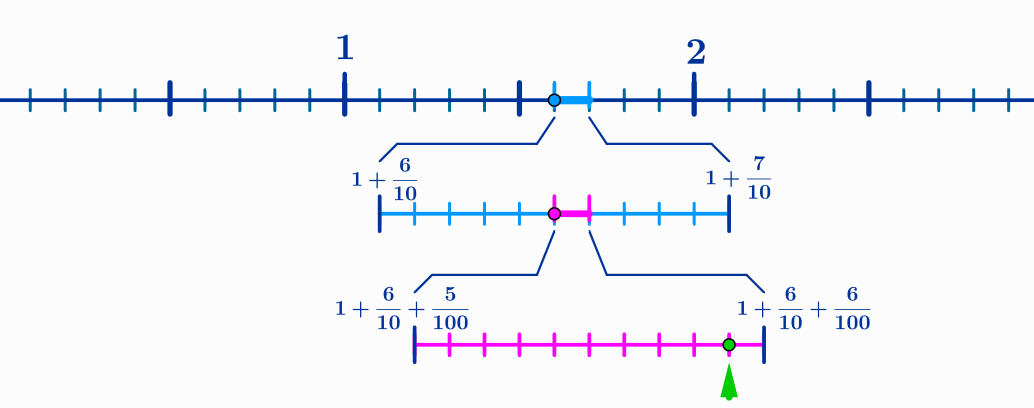
\includegraphics[width=\linewidth]{frac_decimales_demi-droite_zoom.PNG}
\end{center}
\end{Mt}

 

\end{pageCours} 
\begin{pageAD} 
 

\Sf{Connaitre le vocabulaire des opérations}
 
  
\begin{ExoCad}{Communiquer.}{1234}{2}{0}{0}{0}{0}

 \begin{itemize}
 \item Justifier que $\frac{19}{8}=2+\frac{3}{8}$.
 \item Donner un encadrement à l'unité de $\frac{19}{8}$.
 \item Encadrer à l'unité les fractions suivantes.
 \[\frac{7}{2}\hspace{1cm}\frac{9}{4}\hspace{1cm}\frac{5}{3}\]
 \end{itemize}
 
\end{ExoCad}

\Sf{Connaitre les règles de priorités}

\begin{ExoCad}{Calculer.}{1234}{0}{0}{0}{0}{0}


 Compléter le tableau de la même manière que dans l'exemple précédent :
 \begin{center}
 \begin{tabular}{M{5cm}|M{5cm}|M{5cm}}
 Une fraction décimale & Un nombre entier + une fraction décimale & Un nombre entier + des fractions décimales \\\hline\hline
 $\frac{453}{10}$ & & \\\hline
  & $43+\frac{613}{1000}$ & \\\hline
 & & $47+\frac{1}{100}+\frac{9}{1000}$ \\
 \end{tabular}
 \end{center}

 
\end{ExoCad}

\begin{ExoCad}{Calculer.}{1234}{0}{0}{0}{0}{0}

 
\end{ExoCad}


\Sf{Utiliser la distributivité}

\begin{ExoCad}{Représenter. Calculer.}{1234}{0}{0}{0}{0}{0}

 
 
\end{ExoCad}

\begin{ExoCad}{Calculer.}{1234}{0}{0}{0}{0}{0}

 
\end{ExoCad}

 
\end{pageAD}


%%%%%%%%%%%%%%%%%%%%%%%%%%%%%%%%%%%%%%%%%%%%%%%%%%%%%%%%%%%%%%%%%%%
%%%%  Niveau 1
%%%%%%%%%%%%%%%%%%%%%%%%%%%%%%%%%%%%%%%%%%%%%%%%%%%%%%%%%%%%%%%%%%%
\begin{pageParcoursu} 

 %%%%%%%%%%%%%%%%%%%%%%%%%%%
\begin{ExoCu}{Représenter.}{1234}{2}{0}{0}{0}{0}


\end{ExoCu}
%%%%%%%%%%%%%%%%%%%%%%%%%%%
\begin{ExoCu}{Représenter.}{1234}{2}{0}{0}{0}{0}


\end{ExoCu}
%%%%%%%%%%%%%%%%%%%%%%%%%%%
\begin{ExoCu}{Représenter.}{1234}{2}{0}{0}{0}{0}

\end{ExoCu}


%%%%%%%%%%%%%%%%%%%%%%%%%%%
\begin{ExoCu}{Raisonner.}{1234}{2}{0}{0}{0}{0}

\end{ExoCu}

%%%%%%%%%%%%%%%%%%%%%%%%%%%
\begin{ExoCu}{Représenter.}{1234}{2}{0}{0}{0}{0}


\end{ExoCu}


\end{pageParcoursu}

  
%%%%%%%%%%%%%%%%%%%%%%%%%%%%%%%%%%%%%%%%%%%%%%%%%%%%%%%%%%%%%%%%%%%
%%%%  Niveau 2
%%%%%%%%%%%%%%%%%%%%%%%%%%%%%%%%%%%%%%%%%%%%%%%%%%%%%%%%%%%%%%%%%%%



\begin{pageParcoursd} 
 
%%%%%%%%%%%%%%%%%%%%%%%%%%%%%%%%%%%%%%%%%%%%%%%%%%%%%%%%%%%%%%%%%%%
\begin{ExoCd}{Représenter.}{1234}{2}{0}{0}{0}{0}


 
\end{ExoCd}

 
%%%%%%%%%%%%%%%%%%%%%%%%%%%%%%%%%%%%%%%%%%%%%%%%%%%%%%%%%%%%%%%%%%%
\begin{ExoCd}{Chercher.communiquer.}{1234}{2}{0}{0}{0}{0}



\end{ExoCd}


%%%%%%%%%%%%%%%%%%%%%%%%%%%%%%%%%%%%%%%%%%%%%%%%%%%%%%%%%%%%%%%%%%%
\begin{ExoCd}{Représenter. Raisonner.}{1234}{2}{0}{0}{0}{0}


\end{ExoCd}

 %%%%%%%%%%%%%%%%%%%%%%%%%%%%%%%%%%%%%%%%%%%%%%%%%%%%%%%%%%%%%%%%%%%
\begin{ExoCd}{Représenter. Raisonner.}{1234}{2}{0}{0}{0}{0}


\end{ExoCd}
 
%%%%%%%%%%%%%%%%%%%%%%%%%%%%%%%%%%%%%%%%%%%%%%%%%%%%%%%%%%%%%%%%%%%
\begin{ExoCd}{Représenter. Raisonner.}{1234}{2}{0}{0}{0}{0}


\end{ExoCd}
 
\end{pageParcoursd}

%%%%%%%%%%%%%%%%%%%%%%%%%%%%%%%%%%%%%%%%%%%%%%%%%%%%%%%%%%%%%%%%%%%
%%%%  Niveau 3
%%%%%%%%%%%%%%%%%%%%%%%%%%%%%%%%%%%%%%%%%%%%%%%%%%%%%%%%%%%%%%%%%%%
\begin{pageParcourst}

%%%%%%%%%%%%%%%%%%%%%%%%%%%%%%%%%%%%%%%%%%%%%%%%%%%%%%%%%%%%%%%%%%%
\begin{ExoCt}{Représenter.}{1234}{2}{0}{0}{0}{0}

 

\end{ExoCt}

%%%%%%%%%%%%%%%%%%%%%%%%%%%%%%%%%%%%%%%%%%%%%%%%%%%%%%%%%%%%%%%%%%%
\begin{ExoCt}{Représenter. Raisonner.}{1234}{2}{0}{0}{0}{0}
 
 


\end{ExoCt}


%%%%%%%%%%%%%%%%%%%%%%%%%%%%%%%%%%%%%%%%%%%%%%%%%%%%%%%%%%%%%%%%%%%
\begin{ExoCt}{Raisonner.}{1234}{2}{0}{0}{0}{0}
 
\end{ExoCt}

%%%%%%%%%%%%%%%%%%%%%%%%%%%%%%%%%%%%%%%%%%%%%%%%%%%%%%%%%%%%%%%%%%%
\begin{ExoCt}{Représenter.}{1234}{2}{0}{0}{0}{0}

 

\end{ExoCt}

%%%%%%%%%%%%%%%%%%%%%%%%%%%%%%%%%%%%%%%%%%%%%%%%%%%%%%%%%%%%%%%%%%%
\begin{ExoCt}{Représenter.}{1234}{2}{0}{0}{0}{0}

 

\end{ExoCt} 
 
\end{pageParcourst}

%%%%%%%%%%%%%%%%%%%%%%%%%%%%%%%%%%%%%%%%%%%%%%%%%%%%%%%%%%%%%%%%%%%
%%%%  Brouillon
%%%%%%%%%%%%%%%%%%%%%%%%%%%%%%%%%%%%%%%%%%%%%%%%%%%%%%%%%%%%%%%%%%%


\begin{pageBrouillon} 
 
\ligne{32}



\end{pageBrouillon}

%%%%%%%%%%%%%%%%%%%%%%%%%%%%%%%%%%%%%%%%%%%%%%%%%%%%%%%%%%%%%%%%%%%
%%%%  Auto
%%%%%%%%%%%%%%%%%%%%%%%%%%%%%%%%%%%%%%%%%%%%%%%%%%%%%%%%%%%%%%%%%%%


%%%%%%%%%%%%%%%%%%%%%%%%%%%%%%%%%%%%%%%%%%%%%%%%%%%%%%%%%%%%%%%%%%%
\begin{pageAuto} 


\begin{ExoAuto}{Raisonner.}{1234}{2}{0}{0}{0}{0}

 
%%%%%%%%%%%%%%%%%%%%%%%%%%%%%%%%%%%%%%%%%%%%%%%%%%%%%%%%%%%%%%%%%%%
\end{ExoAuto}

\begin{ExoAuto}{Raisonner.}{1234}{2}{0}{0}{0}{0}
  

\end{ExoAuto}

%%%%%%%%%%%%%%%%%%%%%%%%%%%%%%%%%%%%%%%%%%%%%%%%%%%%%%%%%%%%%%%%%%%
\begin{ExoAuto}{Raisonner.}{1234}{2}{0}{0}{0}{0}

 
 

\end{ExoAuto}

 
%%%%%%%%%%%%%%%%%%%%%%%%%%%%%%%%%%%%%%%%%%%%%%%%%%%%%%%%%%%%%%%%%%%
\begin{ExoAuto}{Raisonner.}{1234}{2}{0}{0}{0}{0}

 
 

\end{ExoAuto}


\end{pageAuto}
